\caulc
\begin{ex}%[1D6H4-3]%[TDMZZ17]%[Lê Phúc]
	Tập nghiệm của bất phương trình $\log_{\frac{1}{3}}(x-4)>-2$ là
	\choice
	{\True $(4;13)$}
	{$(4;9)$}
	{$(9;+\infty)$}
	{$(-\infty;13)$}
	\loigiai{
		Điều kiện $x-4>0\Leftrightarrow x>4$.\\
		Ta có
		$\log_{\frac{1}{3}}(x-4)>-2 \Leftrightarrow x-4<\left(\dfrac{1}{3}\right)^{-2}\Leftrightarrow x<13$.\\
		Kết hợp điều kiện ta có $4<x<13$.\\
		Vậy tập nghiệm của bất phương trình là $(4;13)$.
	}
\end{ex}

\begin{ex}%[1D7N2-1]%[TDMZZ17]%[Lê Phúc]
	Biểu thức đạo hàm của hàm số $y=3^x+2\,026$ là
	\choice
	{$y'=\dfrac{3^x}{\ln 3}$}
	{\True $y'=3^x\ln 3$}
	{$y'=3^x$}
	{$y'=3^{x-1}x$}
	\loigiai{
		Ta có $y' = (3^x+2\,026)' = 3^x\ln 3$.
	}
\end{ex}

\begin{ex}%[1D2H3-2]%[TDMZZ17]%[Lê Phúc]
	Cho cấp số nhân $(u_n)$ có $u_1=3$ và $u_4=24$. Công bội của $\left(u_n\right)$ bằng
	\choice
	{$q=2\sqrt{2}$}
	{$q=4$}
	{\True $q=2$}
	{$q=7$}
	\loigiai{
		Ta có $u_4 = u_1\cdot q^3 \Leftrightarrow 24 = 3\cdot q^3 \Leftrightarrow q^3 = 8 \Leftrightarrow q = 2$.
	}
\end{ex}

\begin{ex}%[1H8H6-1]%[TDMZZ17]%[Lê Phúc]
	Cho hình chóp đều $S. ABCD$ có tâm của đáy là $O$. Gọi $\varphi_1$, $\varphi_2$, $\varphi_3$ lần lượt là góc tạo bởi cạnh bên với đáy, cạnh bên với cạnh đáy, mặt bên với mặt đáy. Sắp xếp đúng theo chiều tăng dần là
	\choice
	{$\varphi_1$, $\varphi_2$, $\varphi_3$}
	{$\varphi_3$, $\varphi_1$, $\varphi_2$}
	{\True $\varphi_1$, $\varphi_3$, $\varphi_2$}
	{$\varphi_3$, $\varphi_2$, $\varphi_1$}
	\loigiai{
		\begin{center}
			\begin{tikzpicture}[line join=round, line cap=round,thick]
				\coordinate (A) at (0,0);
				\coordinate (B) at (2,-2);
				\coordinate (D) at (5,0);
				\coordinate (C) at ($(B)+(D)-(A)$);
				\coordinate (O) at ($(A)!0.5!(C)$);
				\coordinate (S) at ($(O)+(0,7)$);
				\coordinate (M) at ($(C)!0.5!(D)$);
				\draw(S)--(A) (S)--(B) (S)--(C) (A)--(B) (B)--(C);
				\draw[dashed](A)--(C) (A)--(D) (C)--(D) (S)--(D) (S)--(O) (B)--(D) (S)--(M)--(O);
				\foreach \i/\g in {S/90,A/180,B/-90,C/-90,D/0,O/-90,M/0}{\draw[fill=black](\i) circle (1pt) ($(\i)+(\g:3mm)$) node[scale=1]{$\i$};}
			\end{tikzpicture}
		\end{center}
		Xét hình chóp đều $S. ABCD$ có đáy $ABCD$ là hình vuông cạnh $a$ ($a > 0$), tâm $O$. \\
		Gọi $M$ là trung điểm của $CD$.
		\begin{itemize}
			\item Góc giữa cạnh bên $SD$ và mặt đáy $(ABCD)$ là $\varphi_1 = \widehat{SDO}$.
			\item Góc giữa mặt bên $(SCD)$ và mặt đáy $(ABCD)$ là $\varphi_3 = \widehat{SMO}$ (vì $SM \perp CD$ và $OM \perp CD$).
			\item Góc giữa cạnh bên $SD$ và cạnh đáy $CD$ là $\varphi_2 = \widehat{SDM}$ (tam giác $SCD$ cân tại $S$).
		\end{itemize}
		Mặt khác, trong các tam giác vuông $SOD$ và $SOM$, ta luôn có $SD > OD$ và $SM > OM$. \\
		Từ đó suy ra $\varphi_1$ và $\varphi_3$ là các góc nhọn.\\
		Trong tam giác vuông $SOD$, ta có $OD = \dfrac{a\sqrt{2}}{2}$ và $SD = \sqrt{SO^2 + OD^2} > OD$.\\
		Trong tam giác vuông $SOM$, ta có $OM = \dfrac{a}{2}$ và $SM = \sqrt{SO^2 + OM^2} > OM$.\\
		\begin{itemize}
			\item $\tan\varphi_1 = \dfrac{SO}{OD} = \dfrac{SO}{\dfrac{a\sqrt{2}}{2}} = \dfrac{2SO}{a\sqrt{2}}$.
			\item $\tan\varphi_3 = \dfrac{SO}{OM} = \dfrac{SO}{\dfrac{a}{2}} = \dfrac{2SO}{a}$.
		\end{itemize}
		Vì $a\sqrt{2} > a > 0$ nên $\dfrac{2SO}{a\sqrt{2}} < \dfrac{2SO}{a} \Rightarrow \tan\varphi_1 < \tan\varphi_3$.\\
		Do $\varphi_1, \varphi_3 \in \left(0^\circ; 90^\circ\right)$ nên $\varphi_1 < \varphi_3$.\\
		\\
		Ta có $\varphi_2 = \widehat{SDM}$ trong tam giác vuông $SMD$ vuông tại $M$
		\[\tan\varphi_2 = \dfrac{SM}{MD} = \dfrac{\sqrt{SO^2 + OM^2}}{OM} = \sqrt{\left(\dfrac{SO}{OM}\right)^2 + 1} = \sqrt{\tan^2\varphi_3 + 1} > \tan\varphi_3.\]
		Do $\varphi_2$, $\varphi_3 \in \left(0^\circ; 90^\circ\right)$ nên $\varphi_2 > \varphi_3$.\\
		Vậy $\varphi_1 < \varphi_3 < \varphi_2$.
	}
\end{ex}

\begin{ex}%[2D1N1-1]%[TDMZZ17]%[Lê Phúc]
	Hàm số $y=\dfrac{x+2}{x-1}$
	\choice
	{\True nghịch biến trên từng khoảng xác định}
	{đồng biến trên từng khoảng xác định}
	{đồng biến trên khoảng xác định}
	{nghịch biến trên tập xác định}
	\loigiai{
		Tập xác định $\mathcal{D} = \mathbb{R} \setminus \{1\}$.\\
		Ta có $y' = \dfrac{1\cdot(-1) - 2\cdot 1}{(x-1)^2} = \dfrac{-3}{(x-1)^2} < 0$, $\forall x \neq 1$.\\
		Do đó hàm số nghịch biến trên từng khoảng xác định $(-\infty;1)$ và $(1;+\infty)$.
	}
\end{ex}

\begin{ex}%[2D4H1-3]%[TDMZZ17]%[Lê Phúc]
	Nếu $C$ là một hằng số thực thì họ nguyên hàm của hàm số $f(x)=\dfrac{2}{x}+\dfrac{1}{\sin^2 x}$ là
	\choice
	{$F(x)=2\ln|x|+\cot x+C$}
	{\True $F(x)=2\ln|x|-\cot x+C$}
	{$F(x)=\ln|x|-\cot x+C$}
	{$F(x)=2\ln|x|-\cos x+C$}
	\loigiai{
		Ta có họ nguyên hàm $\displaystyle\int f(x)\mathrm{\,d}x =\displaystyle\int \left(\dfrac{2}{x}+\dfrac{1}{\sin^2 x}\right)\mathrm{\,d}x = 2\ln|x| - \cot x + C$.
	}
\end{ex}

\begin{ex}%[2H2N2-2]%[TDMZZ17]%[Lê Phúc]
	Trong không gian $Oxyz$, cho điểm $A(1;4;-2)$. Điểm đối xứng với $A$ qua trục $Oy$ có toạ độ là
	\choice
	{$(1;4;-2)$}
	{$(1;0;-2)$}
	{\True $(-1;4;2)$}
	{$(-1;0;2)$}
	\loigiai{
		Điểm đối xứng với $A$ qua trục $Oy$ có toạ độ là $A'(-1;4;2)$.
	}
\end{ex}

\begin{ex}%[2D1H4-1]%[TDMZZ17]%[Lê Phúc]
	Số đường tiệm cận của đồ thị hàm số $y=\dfrac{x+2}{x^2+x-2}$ là
	\choice
	{$3$}
	{$1$}
	{\True $2$}
	{$0$}
	\loigiai{
		Ta có $y=\dfrac{x+2}{(x-1)(x+2)} = \dfrac{1}{x-1}$ (với $x \neq -2$).\\
		Suy ra $\lim\limits_{x\to 2} y=\lim\limits_{x\to 2}\dfrac{1}{x-1}=1$.\\
		Do đó $x=2$ không phải là tiệm cận của đồ thị hàm số.\\
		Ta có $\lim\limits_{x\to \pm\infty} y = 0$.\\
		Suy ra đồ thị hàm số có $1$ tiệm cận ngang là $y = 0$.\\
		Ta có $\lim\limits_{x\to 1^+} y = +\infty$.\\
		Suy ra đồ thị hàm số có $1$ tiệm cận đứng là $x = 1$.\\
		Vậy đồ thị hàm số có $2$ đường tiệm cận.
	}
\end{ex}

\begin{ex}%[2H2H1-2]%[TDMZZ17]%[Lê Phúc]
	Cho hình hộp $ABCD. A'B'C'D'$. Đáp án \textbf{đúng} là
	\choice
	{$\overrightarrow{AB}+\overrightarrow{BB'}+\overrightarrow{B'B}=\overrightarrow{AB'}$}
	{\True $\overrightarrow{CC'}+\overrightarrow{A'D}+\overrightarrow{DB'}=\overrightarrow{AB'}$}
	{$\overrightarrow{AA'}+\overrightarrow{C'C}+\overrightarrow{BB'}=\overrightarrow{AB'}$}
	{$\overrightarrow{AB}+\overrightarrow{AD}+\overrightarrow{AA'}=\overrightarrow{AB'}$}
	\loigiai{
		\immini{Ta có
			$\overrightarrow{CC'} + \overrightarrow{A'D} + \overrightarrow{DB'} = \overrightarrow{AA'} + \overrightarrow{A'B'} = \overrightarrow{AB'}$.}
		{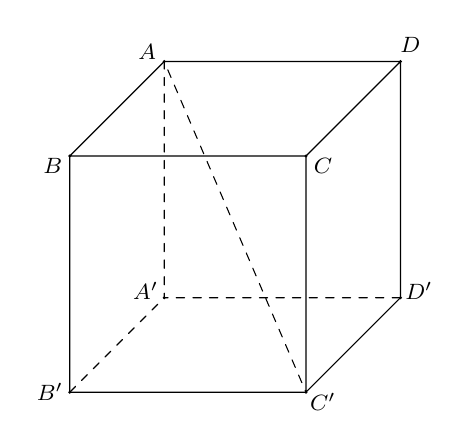
\begin{tikzpicture}[font=\footnotesize,line join=round, line cap=round, >=stealth,scale=0.6] 
				\path 
				(0,0) coordinate (A')
				(-2,-2) coordinate (B')	
				(3,-2) coordinate (C')	
				(5,0) coordinate (D')	
				(0,5) coordinate (A)	
				(-2,3) coordinate (B)	
				(3,3) coordinate (C)	
				(5,5) coordinate (D)
				;
				\draw (B)--(B')--(C')--(C)--(B)--(A)--(D)--(C) (B')--(C')--(D')--(D);
				\draw[dashed] (D')--(A')--(A)--(C') (B')--(A');
				\foreach \x/\pos in{A/150,B/-150,C/-30,D/60,A'/160,B'/180,C'/-30,D'/20}
				\fill (\x) circle(1pt) node[{shift=(\pos:0.25)}]{$\x$}; 
		\end{tikzpicture}}
	}
\end{ex}

\begin{ex}%[1D5H1-3]%[TDMZZ17]%[Lê Phúc]
	Cho hai mẫu số liệu ghép nhóm $M_1$, $M_2$ với bảng tần số ghép nhóm như sau
	\begin{center}
		\begin{tabular}{|c|c|c|c|c|c|c|c|}
			\hline
			\multicolumn{2}{|c|}{Nhóm} & $[5;7)$ & $[7;9)$ & $[9;11)$ & $[11;13)$ & $[13;15)$ & $[15;17)$ \\ \hline
			$M_1$ & Tần số & $3$ & $5$ & $6$ & $4$ & $6$ & $5$ \\ \hline
			$M_2$ & Tần số & $12$ & $10$ & $12$ & $8$ & $12$ & $10$ \\ \hline
		\end{tabular}
	\end{center}
	Hãy so sánh số trung bình cộng $\overline{x_1}$, $\overline{x_2}$ của hai mẫu số liệu $M_1$, $M_2$?
	\choice
	{$\overline{x_1}=\overline{x_2}$}
	{$\overline{x_1}<\overline{x_2}$}
	{\True $\overline{x_1}>\overline{x_2}$}
	{$\overline{x_1}=2\overline{x_2}$}
	\loigiai{
		Bảng giá trị đại diện
		\begin{center}
			\begin{tabular}{|c|c|c|c|c|c|c|c|}
				\hline
				\multicolumn{2}{|c|}{Nhóm} & $[5;7)$ & $[7;9)$ & $[9;11)$ & $[11;13)$ & $[13;15)$ & $[15;17)$ \\ \hline
				\multicolumn{2}{|c|}{Giá trị đại diện} & $6$ & $8$ & $10$ & $12$ & $14$ & $16$ \\ \hline
				$M_1$ & Tần số & $3$ & $5$ & $6$ & $4$ & $6$ & $5$ \\ \hline
				$M_2$ & Tần số & $12$ & $10$ & $12$ & $8$ & $12$ & $10$ \\ \hline
			\end{tabular}
		\end{center}
		\begin{itemize}
			\item \textbf{Với mẫu $M_1$.}\\
			Tổng số số liệu $n_1 = 3+5+6+4+6+5 = 29$.\\
			Số trung bình là
			$\overline{x_1} = \dfrac{3\cdot 6 + 5\cdot 8 + 6\cdot 10 + 4\cdot 12 + 6\cdot 14 + 5\cdot 16}{29} = \dfrac{330}{29} \approx 11{,}38$.
			\item \textbf{Với mẫu $M_2$.}\\
			Tổng số số liệu $n_2 = 12+10+12+8+12+10 = 64$.\\
			Số trung bình là
			$\overline{x_2} = \dfrac{12\cdot 6 + 10\cdot 8 + 12\cdot 10 + 8\cdot 12 + 12\cdot 14 + 10\cdot 16}{64} = \dfrac{696}{64} = 10{,}875$.
		\end{itemize}
		Suy ra $\overline{x_1}> \overline{x_2}$.
	}
\end{ex}

\begin{ex}%[2H5H1-3]%[TDMZZ17]%[Lê Phúc]
	Trong không gian $Oxyz$, cho ba điểm $A(1;2;0)$, $B(-2;1;1)$, $C(3;0;-2)$. Phương trình mặt phẳng đi qua $A$, vuông góc với đường thẳng $BC$ là
	\choice
	{\True $5x-y-3z-3=0$}
	{$x+y-z-3=0$}
	{$2x-y-z=0$}
	{$4x-3y-3z+2=0$}
	\loigiai{
		Vectơ chỉ phương của đường thẳng $BC$ là $\overrightarrow{BC} = (5;-1;-3)$.\\
		Mặt phẳng vuông góc với đường thẳng $BC$ nên nhận $\overrightarrow{n} = \overrightarrow{BC} = (5;-1;-3)$ làm vectơ pháp tuyến.\\
		Phương trình mặt phẳng đi qua $A(1;2;0)$ là
		\[5(x-1) - 1(y-2) - 3(z-0) = 0 \Leftrightarrow 5x - y - 3z - 3 = 0.\]
	}
\end{ex}

\begin{ex}%[2D4H2-2]%[TDMZZ17]%[Lê Phúc]
	Cho tích phân $I=\displaystyle\int\limits_1^2 \dfrac{(x-1)^2}{x}\mathrm{\,d}x = -\dfrac{a}{b}+c\ln 2$; với $a$, $b$, $c$ là những số nguyên dương; phân số $\dfrac{a}{b}$ tối giản. Giá trị của biểu thức $T=a+b+c$ bằng
	\choice
	{$3$}
	{\True $4$}
	{$6$}
	{$7$}
	\loigiai{
		Ta có
		\allowdisplaybreaks
		\begin{eqnarray*}
			I&=&\displaystyle\int\limits_1^2 \dfrac{x^2-2x+1}{x}\mathrm{\,d}x\\
			&=&\displaystyle\int\limits_1^2 \left(x - 2 + \dfrac{1}{x}\right)\mathrm{\,d}x\\
			&=&\left.\left(\dfrac{x^2}{2} - 2x + \ln|x|\right)\right|_1^2\\
			&=&\left(\dfrac{4}{2} - 4 + \ln 2\right) - \left(\dfrac{1}{2} - 2 + \ln 1\right)\\
			&=&-\dfrac{1}{2} + \ln 2.
		\end{eqnarray*}
		Suy ra $a=1$, $b=2$, $c=1$.\\
		Khi đó $T = a+b+c = 1+2+1 = 4$.
	}
\end{ex}
\cauds
\begin{ex}%[2D4H2-6]%[Dương Công Tạo]
	Cho một vật bắt đầu chuyển động thẳng với biểu thức gia tốc là \[a(t) = \heva{&1{,}8 && \text{ nếu } 0 \le t \le 20 \\ &21{,}8-t && \text{ nếu } t > 20}\;\left(\mathrm{m/s^2}\right).\] Biết rằng khi vật đang chuyển động mà chuyển động chậm dần cho đến khi vận tốc bằng $0$ thì vật sẽ dừng hẳn.
	\choiceTF
	{\True Gia tốc của vật ở thời điểm $21$ giây bằng $0{,}8$ (m/s$^2$)}
	{Biểu thức vận tốc của vật $v(t) = \heva{&2t & \text{ nếu } 0 \le t \le 20 \\&21{,}8t-0{,}5t^2 & \text{ nếu } 10 < t < 15}$}
	{\True Quãng đường vật đi được trong $20$ giây đầu tiên là $360$ (m)}
	{Tổng quãng đường vật đi được tính từ lúc bắt đầu chuyển động cho tới khi dừng lại là $640$ mét (\textit{làm tròn kết quả đến hàng đơn vị})}
	\loigiai{
		\begin{itemchoice}
			\itemch Gia tốc của vật ở thời điểm $21$ giây là $a(21)=21{,}8-21=0{,}8$ (m/s$^2$).
			\itemch \begin{itemize}
				\item Với $0\leq t\leq 20$, ta có $v_1(t)=\displaystyle\int{1{,}8}\,\mathrm{d}t=1{,}8t+C$.\\
				Vì $v(0)=0$ nên $C=0$. Suy ra $v(t)=1{,}8t$.
				\item Với $t>20$, ta có $v(t)=\displaystyle\int{(21{,}8-t)}\,\mathrm{d}t=21{,}8t-\dfrac{1}{2}t^2+D$.\\
				Vì $v_1(20)=1{,}8\cdot 20=36=v_2(20)$ (do hàm số liên tục tại $x=20$) nên $D=-200$. \\
				Suy ra $v_2(t)=21{,}8t-\dfrac{1}{2}t^2-200$.
			\end{itemize}
			Vậy biểu thức vận tốc của vật $v(t) = \heva{&1{,}8t & \text{ nếu } 0 \le t \le 20 \\&21{,}8t-0{,}5t^2-200 & \text{ nếu } t>20.}$
			\itemch Quãng đường vật đi được trong $20$ giây đầu tiên là $s_1=\displaystyle\int\limits_0^{20}{1{,}8}t\,\mathrm{d}t=360$ (m).
			\itemch Vật dừng hẳn khi $v_2(t)=0\Leftrightarrow 21{,}8t-0{,}5t^2-200=0\Leftrightarrow \hoac{&t\approx30{,}5&\text{ (nhận)}\\&t\approx13{,}1&\text{ (loại).}}$\\
			Khi đó, quãng đường đi được trong khoảng thời gian này là \[s_2=\displaystyle\int\limits_0^{30{,}5}{\left(21{,}8t-0{,}5t^2-200\right)}\,\mathrm{d}t\approx 284\;(\mathrm{m}).\]
			Vậy, tổng quãng đường vật đi được tính từ lúc bắt đầu chuyển động cho tới khi dừng lại là $360+284=644$ (m).
		\end{itemchoice}
	}
\end{ex}

\begin{ex}%[TDMZZ17-14-DS]%[Hà Văn Hảo]%[2D1V5-8]
	\immini[thm]{Trong mùa mưa lũ, nước ở trên thượng nguồn đổ dồn về hạ lưu rất mạnh nên thường làm lệch quỹ đạo chuyển động của tàu, thuyền trên sông. Giả sử trong một hệ trục tọa độ $Oxy$ cho trước có đơn vị dài trên mỗi trục là $500$ mét, có một chiếc thuyền đang ở tại điểm $A(5;3)$ và chuyển động về phía gốc tọa độ $O$. Do dòng chảy mạnh nên thuyền di chuyển trên cung đường $AB$ là một phần của đồ thị hàm số $y=\dfrac{ax+b}{cx+d}$ như hình vẽ, với $B(-1;0)$, giao điểm của đồ thị hàm số với trục tung là $\left(0;\dfrac{8}{5}\right)$.}{
		\begin{tikzpicture}[>=stealth,line join=round,line cap=round,every node/.style={font=\normalsize}]
			\tikzset{
				declare function={
					f (\x) = (40*\x+40)/(11*\x+25);
					xmin = -1.8;
					xmax = 6.2;
					ymin = -0.8;
					ymax = 4.2;
				},
				boat/.pic={
					\draw[line width=0.6pt,fill=gray!20] (-0.6,0.15) -- (-0.4,0) -- (0.4,0) -- (0.7,0.15) -- cycle;
					\draw[line width=1.2pt,blue] (-0.5,0.07) -- (0.55,0.07);
					\draw[line width=0.8pt,brown] (0.1,0.15) -- (0.1,1.4);
					\draw[line width=0.6pt,fill=white] (0.05,0.2) -- (0.05,1.1) -- (-0.55,0.2) -- cycle;
					\draw[line width=0.6pt,fill=white] (0.15,0.2) -- (0.15,1.3) -- (0.6,0.2) -- cycle;
					\fill[red] (0.1,1.4) -- (0.35,1.35) -- (0.1,1.3) -- cycle;
				}
			}
			\draw[-Stealth,line width=0.7pt] (xmin,0) -- (xmax,0) node[below] {$x$};
			\draw[-Stealth,line width=0.7pt] (0,ymin) -- (0,ymax) node[right] {$y$};
			\draw[line width=0.6pt] (-1,-2pt) -- (-1,2pt);
			\node[below] at (-1,-2pt) {$-1$};
			\foreach \x in {1,2,3,4,5}{
				\draw[line width=0.6pt] (\x,-2pt) -- (\x,2pt);
				\node[below] at (\x,-2pt) {$\x$};
			}
			\draw[line width=0.6pt] (-2pt,-0.5) -- (2pt,-0.5);
			%	\node[left] at (-2pt,-0.5) {$-0.5$};
			\foreach \y in {1,2,3}{
				\draw[line width=0.6pt] (-2pt,\y) -- (2pt,\y);
				\node[left] at (-2pt,\y) {$\y$};
			}
			\node[below left] at (0,0) {$0$};
			%	\node[below right] at (0.1,0) {$O (0; 0)$};
			\begin{scope}
				\clip (xmin,ymin) rectangle (xmax,ymax);
				\draw[line width=0.6pt,color=green!50!black,smooth,samples=200,domain=-1:5.5] plot (\x,{f (\x)});
			\end{scope}
			\draw[dashed,line width=0.6pt] (5,0) -- (5,3) -- (0,3);
			\draw[dashed,line width=0.6pt] (0,0) -- (2.5,{f (2.5)});
			\path (5,3) pic {boat};
			\fill (-1,0) circle (1pt) node[above left] {$B (-1; 0)$};
			\fill (0,1.6) circle (1pt);
			\fill (2.5,{f (2.5)}) circle (1pt) node[below right] {$M$};
			\fill (5,3) circle (1pt) node[below right] {$A (5; 3)$};
			\fill (5,0) circle (1pt);
			\fill (0,3) circle (1pt);
			\fill (0,0) circle (1pt);
		\end{tikzpicture}
	}
	\choiceTF
	{\True $a=b$}
	{\True $\dfrac{b}{d}=\dfrac{8}{5}$}
	{$c=\dfrac{3a}{10}$}
	{\True Khi thuyền có hoành độ bằng $1$ thì nó cách gốc $O$ một đoạn bằng $1\,218$ mét (\textit{tính theo đơn vị mét và làm tròn kết quả đến hàng đơn vị})}
	\loigiai{
		Đồ thị hàm số $y=\dfrac{ax+b}{cx+d}$ ($ad-bc \neq 0, c \neq 0$) đi qua các điểm đã cho
		\begin{itemize}
			\item Đi qua $B(-1;0) \Rightarrow 0 = \dfrac{-a+b}{-c+d} \Rightarrow -a+b = 0 \Rightarrow a = b$.
			\item Đi qua giao điểm với trục tung $\left(0;\dfrac{8}{5}\right) \Rightarrow \dfrac{b}{d} = \dfrac{8}{5} \Rightarrow b = \dfrac{8}{5}d$.
			\item Đi qua $A(5;3) \Rightarrow 3 = \dfrac{5a+b}{5c+d}$.
		\end{itemize}
		Từ $a=b$ và $b=\dfrac{8}{5}d$, ta chọn $d=5 \Rightarrow a = b = 8$. Thay vào phương trình đi qua $A$
		\[3 = \dfrac{5 \cdot 8 + 8}{5c + 5} \Rightarrow 3(5c+5) = 48 \Rightarrow 15c + 15 = 48 \Rightarrow 15c = 33 \Rightarrow c = \dfrac{11}{5}.\]
		Vậy hàm số có dạng $y = \dfrac{8x+8}{\dfrac{11}{5}x+5} = \dfrac{40x+40}{11x+25}$.
		\begin{itemchoice}
			\itemch Từ phương trình $-a+b=0$ ta có $a=b$.
			\itemch Thay $x=0$ vào hàm số ta được $y=\dfrac{b}{d}$. Theo giả thiết giao điểm với trục tung là $\dfrac{8}{5}$ nên $\dfrac{b}{d}=\dfrac{8}{5}$.
			\itemch Ta có $a=8$ và $c=\dfrac{11}{5}$. Kiểm tra biểu thức $\dfrac{3a}{10} = \dfrac{3 \cdot 8}{10} = \dfrac{12}{5} \neq \dfrac{11}{5}$.
			\itemch Khi thuyền có hoành độ $x=1$, tung độ của thuyền là
			\[y = \dfrac{40 \cdot 1 + 40}{11 \cdot 1 + 25} = \dfrac{80}{36} = \dfrac{20}{9}.\]
			Khoảng cách từ thuyền đến gốc tọa độ $O$ trong hệ trục là
			\[d_0 = \sqrt{x^2+y^2} = \sqrt{1^2 + \left(\dfrac{20}{9}\right)^2} = \sqrt{1 + \dfrac{400}{81}} = \sqrt{\dfrac{481}{81}} = \dfrac{\sqrt{481}}{9} \approx 2{,}4369 \text{ (đơn vị dài)}.\]
			Vì mỗi đơn vị dài trên trục tương ứng với $500$ mét, khoảng cách thực tế là
			\[d = 2{,}4369 \cdot 500 \approx 1\,218{,}45 \text{ mét} \approx 1\,218 \text{ mét}.\]
		\end{itemchoice}
	}
\end{ex}

\begin{ex}%[2D6C2-4]%[TDMZZ17]%[Vũ Hồng Toàn]
	Mùa $2025$–$2026$ giải ngoại hạng Anh có $20$ đội bóng tham dự và sau vòng $36$ đấu bảng xếp hạng được cho như hình vẽ bên dưới. Hiện tại đội \textbf{Liverpool} đang xếp vị trí thứ $5$. Giả sử trong trận đấu sắp tới nếu gặp đội bên trên bảng xếp hạng thì \textbf{Liverpool} có xác suất thắng là $0{,}3$; xác suất thua là $0{,}3$. Nếu gặp đội bên dưới thì \textbf{Liverpool} có xác suất thắng là $0{,}6$ và xác suất hoà là $0{,}3$. Giả sử: tiến hành bốc thăm ngẫu nhiên một đội đấu với đội \textbf{Liverpool} trong trận tới. Gọi $A$ là biến cố đội \textbf{Liverpool} thắng ở trận đấu tới, $B$ là biến cố đội \textbf{Liverpool} hoà ở trận đấu tới, $C$ là biến cố đội \textbf{Liverpool} gặp đội bên trên.
	\begin{center}
		\begin{tikzpicture}[scale=1.2,
			every node/.style={font=\normalsize},
			declare function={
				rowH = 0.8;
				colRank = 0;
				colLogo = 0.6;
				colName = 1.1;
				colP = 5.5;
				colW = 6.3;
				colD = 7.1;
				colL = 7.9;
				colGF = 8.7;
				colGA = 9.5;
				colGD = 10.3;
				colPts = 11.1;
				colForm = 13.0;
				formStart = 12.2;
				formStep = 0.4;
				lineL = -0.6;
				lineR = 14.2;
				boxL = -0.5;
			}
			]
			\draw[cyan!60,line width=2pt] (lineL,-0.5*rowH) -- (lineL,-4.5*rowH);
			\draw[orange!80,line width=2pt] (lineL,-4.5*rowH) -- (lineL,-5.5*rowH);
			\draw[green!60!black,line width=2pt] (lineL,-5.5*rowH) -- (lineL,-6.5*rowH);
			\foreach \i in {0,1,2,3,4,5,6,7,8,9,10}{
				\draw[gray!30,line width=0.4pt] (lineL,-\i*rowH - 0.5*rowH) -- (lineR,-\i*rowH - 0.5*rowH);
			}
			\node[anchor=west,text=gray!80!black] at (-0.1,0) {Câu lạc bộ};
			\node[text=gray!80!black] at (colP,0) {ĐĐ};
			\node[text=gray!80!black] at (colW,0) {Thắng};
			\node[text=gray!80!black] at (colD,0) {H};
			\node[text=gray!80!black] at (colL,0) {Thua};
			\node[text=gray!80!black] at (colGF,0) {BT};
			\node[text=gray!80!black] at (colGA,0) {SBT};
			\node[text=gray!80!black] at (colGD,0) {HS};
			\node[font=\bfseries] at (colPts,0) {Đ};
			\node[text=gray!80!black] at (colForm,0) {5 trận gần nhất};
			\foreach \rank/\logoC/\logoText/\team/\p/\w/\d/\l/\gf/\ga/\gd/\pts/\fA/\fB/\fC/\fD/\fE in {
				1/red!80!black/A/Arsenal/36/24/7/5/68/26/42/79/2/2/1/1/1,
				2/cyan!50/M/Man City/36/23/8/5/75/32/43/77/1/1/3/1/1,
				3/red!80!black/M/Man Utd/36/18/11/7/63/48/15/65/2/1/1/1/3,
				4/purple!80!black/A/Aston Villa/37/18/8/11/54/48/6/62/1/2/2/3/1,
				5/red/L/Liverpool/37/17/8/12/62/52/10/59/1/1/2/3/2,
				6/black/B/Bournemouth/36/13/16/7/56/52/4/55/1/1/3/1/1,
				7/blue!70!cyan/B/Brighton/36/14/11/11/52/42/10/53/1/3/1/2/1,
				8/red!70/B/Brentford/36/14/9/13/52/49/3/51/3/3/2/1/2,
				9/blue!80/C/Chelsea/36/13/10/13/55/49/6/49/2/2/2/2/3,
				10/blue!60!black/E/Everton/36/13/10/13/46/46/0/49/3/2/2/3/3
			}{
				\pgfmathsetmacro{\y}{-\rank*rowH}
				\node[text=black!80] at (colRank,\y) {\rank};
				\fill[\logoC] (colLogo,\y) circle (0.18);
				\node[text=white,font=\tiny\sffamily\bfseries] at (colLogo,\y) {\logoText};
				\node[anchor=west,text=black!80] at (colName,\y) {\team};
				\node[text=black!80] at (colP,\y) {\p};
				\node[text=black!80] at (colW,\y) {\w};
				\node[text=black!80] at (colD,\y) {\d};
				\node[text=black!80] at (colL,\y) {\l};
				\node[text=black!80] at (colGF,\y) {\gf};
				\node[text=black!80] at (colGA,\y) {\ga};
				\node[text=black!80] at (colGD,\y) {\gd};
				\node[font=\bfseries] at (colPts,\y) {\pts};
				\foreach \f/\i in {\fA/0,\fB/1,\fC/2,\fD/3,\fE/4}{
					\pgfmathsetmacro{\x}{formStart + \i*formStep}
					\ifnum\f=1
					\fill[green!60!black] (\x,\y) circle (0.16);
					\draw[white,thick,line cap=round,line join=round] (\x - 0.06,\y) -- (\x - 0.02,\y - 0.06) -- (\x + 0.06,\y + 0.06);
					\fi
					\ifnum\f=2
					\fill[red!70!black] (\x,\y) circle (0.16);
					\draw[white,thick,line cap=round] (\x - 0.06,\y - 0.06) -- (\x + 0.06,\y + 0.06);
					\draw[white,thick,line cap=round] (\x - 0.06,\y + 0.06) -- (\x + 0.06,\y - 0.06);
					\fi
					\ifnum\f=3
					\fill[gray] (\x,\y) circle (0.16);
					\draw[white,thick,line cap=round] (\x - 0.06,\y) -- (\x + 0.06,\y);
					\fi
				}
			}
			\draw[cyan,line width=1.5pt] (boxL,-5.5*rowH) rectangle (lineR,-4.5*rowH);
		\end{tikzpicture}
	\end{center}
	\choiceTF
	{Xác suất để Liverpool gặp đội xếp trên là $\mathrm{P}(C) = \dfrac{1}{5}$}
	{\True Xác suất để Liverpool thắng ở trận đấu tới là $\mathrm{P}(A) = \dfrac{51}{95}$}
	{\True Xác suất để Liverpool hoà ở trận đấu tới là $\mathrm{P}(B) = \dfrac{61}{190}$}
	{Nếu biết trận đấu tới kết thúc với tỉ số hoà, xác suất để Liverpool đã gặp đội xếp trên là $\mathrm{P}(C\mid B) = \dfrac{4}{15}$}
	\loigiai{
		\begin{itemchoice}
			\itemch Số đội xếp trên Liverpool là $4$ đội (vị trí từ $1$ đến $4$).\\
			Số đội xếp dưới Liverpool là $20 - 5 = 15$ đội (vị trí từ $6$ đến $20$).\\
			Khi bốc thăm ngẫu nhiên một đội đấu với Liverpool, tổng số đối thủ có thể gặp là $19$ đội.\\
			Vậy, xác suất của biến cố $C$ là $\mathrm{P}(C) = \dfrac{4}{19}$.
			\itemch Xác suất của biến cố \lq\lq đội Liverpool gặp đội bên dưới\rq\rq~ là $\mathrm{P}\left(\overline{C}\right) = 1 - \mathrm{P}(C) = \dfrac{15}{19}$.
			\begin{itemize}
				\item Nếu gặp đội bên trên
				\begin{itemize}
					\item Xác suất thắng là $\mathrm{P}(A\mid C) = 0{,}3$.
					\item Xác suất thua là $\mathrm{P}(\text{thua}\mid C) = 0{,}3$.
					\item Xác suất hoà là $\mathrm{P}(B\mid C) = 1 - 0{,}3 - 0{,}3 = 0{,}4$.
				\end{itemize}
				\item Nếu gặp đội bên dưới
				\begin{itemize}
					\item Xác suất thắng là $\mathrm{P}\left(A\mid \overline{C}\right) = 0{,}6$.
					\item Xác suất hoà là $\mathrm{P}\left(B\mid \overline{C}\right) = 0{,}3$.
				\end{itemize}
			\end{itemize}
			Do đó, xác suất để Liverpool thắng ở trận đấu tới là
			\[\mathrm{P}(A) = \mathrm{P}(C) \cdot \mathrm{P}(A\mid C) + \mathrm{P}\left(\overline{C}\right) \cdot \mathrm{P}\left(A\mid \overline{C}\right) = \dfrac{4}{19} \cdot 0{,}3 + \dfrac{15}{19} \cdot 0{,}6 = \dfrac{51}{95}.\]
			\itemch Xác suất để Liverpool hoà ở trận đấu tới là
			\[\mathrm{P}(B) = \mathrm{P}(C) \cdot \mathrm{P}(B\mid C) + \mathrm{P}\left(\overline{C}\right) \cdot \mathrm{P}\left(B\mid \overline{C}\right) = \dfrac{4}{19} \cdot 0{,}4 + \dfrac{15}{19} \cdot 0{,}3 = \dfrac{61}{190}.\]
			\itemch Theo công thức Bayes, ta có
			\[\mathrm{P}(C\mid B) = \dfrac{\mathrm{P}(C \cap B)}{\mathrm{P}(B)} = \dfrac{\mathrm{P}(C) \cdot \mathrm{P}(B\mid C)}{\mathrm{P}(B)} = \dfrac{\dfrac{4}{19} \cdot 0{,}4}{\dfrac{61}{190}} = \dfrac{16}{61}.\]
		\end{itemchoice}
	}
\end{ex}

\begin{ex}%[2H5V3-4]%[TDMZZ17]%[Văn Minh Thoại]
	Trong không gian $Oxyz$ có đơn vị dài trên mỗi trục là mét, có một quả cầu đặc bằng thép có tâm $O$ và có bán kính bằng $120$ cm, một nguồn phát sóng âm đặt tại $A(6;8;0)$. Biết sóng âm truyền thẳng từ nguồn $A$ với tốc độ là $340$ m/s.
	\choiceTF
	{\True $OA=10$ mét}
	{Tất cả các điểm $M(x;y;z)$ thuộc quả cầu đều thoả mãn $x^2+y^2+z^2<1{,}44$}
	{Khoảng thời gian lớn nhất để sóng âm đi từ $A$ đến bề mặt quả cầu là $29$ mili giây \textit{(tính theo đơn vị mili giây và làm tròn kết quả đến hàng đơn vị)}}
	{\True Khi sóng âm truyền theo phương $\overrightarrow{u}=(-6;-8;1)$ thì khoảng thời gian để nó truyền từ $A$ đến bề mặt quả cầu là $27$ mili giây \textit{(tính theo đơn vị mili giây và làm tròn kết quả đến hàng đơn vị)}}
	\loigiai{
		Đổi đơn vị $R=120$ cm$=1{,}2$ m. Tọa độ tâm quả cầu là $O(0;0;0)$.
		\begin{itemchoice}
			\itemch Ta có $OA=\sqrt{6^2+8^2+0^2}=10$ m.
			\itemch Quả cầu đặc bao gồm cả phần bên trong và bề mặt, do đó tập hợp tất cả các điểm $M(x;y;z)$ thuộc quả cầu là một khối cầu, phải thỏa mãn điều kiện
			\allowdisplaybreaks
			\begin{eqnarray*}
				&&OM\le R\\
				&\Leftrightarrow& x^2+y^2+z^2\le 1{,}2^2\\
				&\Leftrightarrow& x^2+y^2+z^2\le 1{,}44.
			\end{eqnarray*}
			Vậy tất cả các điểm $M(x;y;z)$ thuộc quả cầu đều thoả mãn $x^2+y^2+z^2\le1{,}44$
			\itemch Khoảng cách lớn nhất từ $A$ đến bề mặt quả cầu là đoạn $\mathrm{d}_{\max}=OA+R=10+1{,}2=11{,}2$ m. \\
			Khoảng thời gian lớn nhất tương ứng là
			\[t_{\max} =\dfrac{\mathrm{d}_{\max}}{v}=\dfrac{11{,}2}{340} \approx 0{,}03294\mathrm{\,s}\approx 33 \mathrm{\,ms}\ne29\mathrm{\,ms}.\]
			\itemch
			\begin{center}
				\begin{tikzpicture}[line join=round,line cap=round,>=stealth,scale=1]
					\tdplotsetmaincoords{70}{110}
					\def\R{2} % ban kinh mat cau
					\def\xA{6} % hoanh do diem A
					\def\yA{8} % tung do diem A
					\pgfmathsetmacro{\dA}{sqrt (\xA*\xA+\yA*\yA)}
					\pgfmathsetmacro{\can}{sqrt (\R*\R*(\dA*\dA+1)-\dA*\dA)}
					\pgfmathsetmacro{\tMot}{(\dA*\dA-\can)/(\dA*\dA+1)}
					\pgfmathsetmacro{\tHai}{(\dA*\dA+\can)/(\dA*\dA+1)}
					\draw (0,0) circle[radius=\R];
					
					\begin{scope}[tdplot_main_coords]
						\coordinate (O) at (0,0,0);
						\coordinate (A) at (\xA,\yA,0);
						\coordinate (Ax) at (\xA,0,0);
						\coordinate (Ay) at (0,\yA,0);
						\coordinate (M) at ({\xA*(1-\tMot)},{\yA*(1-\tMot)},{\tMot});
						\coordinate (M2) at ({\xA*(1-\tHai)},{\yA*(1-\tHai)},{\tHai});
						\coordinate (P) at ({\R*\xA/\dA},{\R*\yA/\dA},0);
						\coordinate (Mmax) at ({-\R*\xA/\dA},{-\R*\yA/\dA},0);
						\draw[dashed] (O) -- (\R+2.3,0,0);
						\draw[->] (\R+2.3,0,0) -- ({\xA+1.5},0,0)
						node[below left] {$x$};
						\draw[dashed] (O) -- (0,\R,0);
						\draw[->] (0,\R,0) -- (0,{\yA+1.5},0)
						node[right] {$y$};
						\draw[dashed] (O) -- (0,0,\R);
						\draw[->] (0,0,\R) -- (0,0,{\R+1.5})
						node[above] {$z$};
						\draw[dashed] plot[domain=100:300,samples=100]
						({\R*cos (\x)},{\R*sin (\x)},0);
						\draw plot[domain=300:460,samples=100]
						({\R*cos (\x)},{\R*sin (\x)},0);
						\draw[dashed] (Ax) -- (A) -- (Ay);
						\draw (A) -- (P);
						\draw[dashed] (P) -- (Mmax);
						\draw (A) -- (M);
						\draw[->] (A) -- ($(A)!0.4!(M)$) node[pos=0.5,sloped,above] {$\overrightarrow{u}$};
						
						\draw[dashed] (M) -- (M2);
						\path (O) -- (Mmax) node[pos=0.5,sloped,below] {$R$};
						
						\foreach \p/\goc/\ten in {
							O/-90/O,
							A/-90/A,
							M/210/M,
							Mmax/120/M_{\max}}{\draw[fill,ball color=red] (\p) circle (1pt) node[shift={(\goc:9pt)},font=\scriptsize] {$\ten$};}
						\draw[fill,ball color=red] (Ax) circle (1pt) node[shift={(160:9pt)}] {$\xA$};
						\draw[fill,ball color=red] (Ay) circle (1pt) node[shift={(90:9pt)}] {$\yA$};
					\end{scope}
				\end{tikzpicture}
			\end{center}
			Đường thẳng $\Delta$ biểu diễn phương truyền sóng đi qua $A(6;8;0)$ và có một vectơ chỉ phương $\overrightarrow{u}=(-6;-8;1)$. Phương trình tham số của $\Delta$ là
			$\heva{&x=6-6t\\&y=8-8t\\&z=t}\quad(t>0)$.\\
			Tọa độ giao điểm $M$ của sóng với bề mặt quả cầu có phương là $x^2+y^2+z^2=1{,}44$, khi đó
			\allowdisplaybreaks
			\begin{eqnarray*}
				&&(6 - 6t)^2 + (8 - 8t)^2 + t^2= 1{,}44 \\
				&\Leftrightarrow& 36(1 - t)^2 + 64(1 - t)^2 + t^2= 1{,}44 \\
				&\Leftrightarrow& 100(1 - t)^2 + t^2= 1{,}44 \\
				&\Leftrightarrow& 101t^2 - 200t + 98{,}56= 0\\
				&\Leftrightarrow& \heva{&t_1\approx 0{,}9234 \\&t_2\approx 1{,}0568.}
			\end{eqnarray*}
			Sóng gặp bề mặt quả cầu lần đầu tiên tại điểm ứng với thời gian ngắn nhất, tức là $t=t_1$.\\
			Quãng đường sóng truyền từ $A$ đến bề mặt quả cầu là $\mathrm{d}=AM$, Khi đó
			\[AM = \sqrt{(-6t)^2 + (-8t)^2 + t^2} = t\sqrt{101} \approx 0{,}9234 \cdot \sqrt{101} \approx 9{,}279\; \mathrm{m}.\]
			Khoảng thời gian để sóng truyền tới bề mặt quả cầu là
			\[\Delta t = \dfrac{\mathrm{d}}{v} = \dfrac{9{,}279}{340} \approx 0{,}02729 \mathrm{\,s}\approx 27\mathrm{\,ms}.\]
		\end{itemchoice}
	}
\end{ex}
\caukq
\begin{ex}%[2D1H5-8]%[TDMZZ17]%[Lê Hồ Quang Minh]
	Giả sử số lượng tế bào của một quần thể nấm men tại một môi trường nuôi cấy trong phòng thí nghiệm được mô hình hoá bằng hàm số $P(t) = \dfrac{a}{b + \mathrm{e}^{-0,5t}}$, trong đó thời gian $t$ được tính theo giờ. Tại thời điểm ban đầu $t = 0$, quần thể có $60$ tế bào và tốc độ sinh trưởng là $20$ tế bào/giờ. Hỏi sau bao nhiêu giờ thì tốc độ sinh trưởng của quần thể nấm men đạt mức tối đa \textit{(không làm tròn các phép tính trung gian và làm tròn kết quả cuối cùng đến hàng phần trăm)}?
	\par\shortans[oly]{1,39}
	\loigiai{
		Tốc độ sinh trưởng của quần thể tại thời điểm $t$ là
		\[P'(t) = \dfrac{a \cdot 0{,}5\mathrm{e}^{-0,5t}}{\left(b + \mathrm{e}^{-0{,}5t}\right)^2}.\]
		Theo giả thiết ta có
		\[\heva{&P(0) = 60 \\ &P'(0) = 20} \Leftrightarrow \heva{&\dfrac{a}{b + 1} = 60 \\ &\dfrac{0{,}5a}{(b + 1)^2} = 20} \Rightarrow \heva{&b = 0{,}5 \\ &a = 90.}\]
		Khi đó $P'(t) = \dfrac{45\mathrm{e}^{-0{,}5t}}{\left(0{,}5 + \mathrm{e}^{-0{,}5t}\right)^2}$.\\
		Ta có
		\allowdisplaybreaks
		\begin{eqnarray*}
			P''(t) &=& \dfrac{-22{,}5\mathrm{e}^{-0{,}5t}\cdot \left(0{,}5 + \mathrm{e}^{-0{,}5t}\right)^2 - 2\cdot \left(0{,}5 + \mathrm{e}^{-0{,}5t}\right)\cdot \left(-0{,}5\mathrm{e}^{-0{,}5t}\right)\cdot 45\mathrm{e}^{-0{,}5t}}{\left(0{,}5 + \mathrm{e}^{-0{,}5t}\right)^4}\\
			&=& \dfrac{-22{,}5\mathrm{e}^{-0{,}5t}\cdot \left(0{,}5 + \mathrm{e}^{-0{,}5t}\right) - 2\cdot \left(-0{,}5\mathrm{e}^{-0{,}5t}\right)\cdot 45\mathrm{e}^{-0{,}5t}}{\left(0{,}5 + \mathrm{e}^{-0{,}5t}\right)^3}\\
			&=& \dfrac{-22{,}5\mathrm{e}^{-0{,}5t}\cdot \left(0{,}5 - \mathrm{e}^{-0{,}5t}\right)}{\left(0{,}5 + \mathrm{e}^{-0{,}5t}\right)^3}.
		\end{eqnarray*}
		Cho $P''(t) = 0 \Leftrightarrow 0{,}5 - \mathrm{e}^{-0{,}5t} = 0 \Leftrightarrow \mathrm{e}^{-0{,}5t} = 0{,}5 \Leftrightarrow t = 2\ln 2$.\\
		Bảng biến thiên
		\begin{center}
			
\begin{tikzpicture}
				\tkzTabInit[nocadre=false,lgt=1.5,espcl=2.5,deltacl=0.6]
				{$t$/0.7,$P''(t)$/0.7,$P'(t)$/1.5}{$0$,$2\ln2$,$+\infty$}
				\tkzTabLine{,+,0,-,}   
				\tkzTabVar{-/,+/$P'\left(2\ln2\right)$,-/}
			\end{tikzpicture}
		\end{center}
		Vậy tốc độ sinh trưởng đạt mức tối đa tại thời điểm $t = 2\ln 2 \approx 1,39$ (giờ).
	}
\end{ex}
\begin{ex}%[Duong Xuan Loi]%[1H8V6-2]
	Cho hình chóp $S.ABC$ có $AB=4$, $AC=6$, $\widehat{BAC}=60^\circ$ và chiều dài cạnh bên $SA=5$. Biết hình chiếu vuông góc của $S$ trên đáy $(ABC)$ nằm trong đoạn $AM$, với $M$ là trung điểm của cạnh $BC$, $\mathrm{d}(S,(ABC))=3$. Hãy xác định số đo góc nhị diện $[S,BC,A]$ theo đơn vị độ (\textit{làm tròn kết quả đến hàng đơn vị})?
	\shortans{$84$}
	\loigiai{
		\begin{center}
			\begin{tikzpicture}[scale=1,line join=round,line cap=round,font=\footnotesize,>=stealth]
				\path 
				(0,0) coordinate (A)
				(1,-1.4) coordinate (B)
				(4.5,0) coordinate (C)
				($(C)!0.5!(B)$) coordinate (M)
				($(A)!0.65!(M)$) coordinate (H)				
				($(H)+(0,3)$) coordinate (S)	
				($(B)!0.19!(C)$) coordinate (K)	
				($(K)+(H)-(A)$) coordinate (I)					
				(intersection of H--I and B--C) coordinate (E)
				;
				\draw (A)--(B)--(C)--(S)--cycle (E)--(S)--(B);
				\draw[dashed] (M)--(A)--(C) (S)--(H)--(E) (A)--(K);
				\foreach \p/\q in {S/90,A/180,B/-90,C/0,M/-30,H/20,K/-40,E/-40}
				\fill[black] (\p) circle (1.0pt) ($(\p)+(\q:3mm)$) node{$\p$};		
			\end{tikzpicture}
		\end{center}
		Gọi $H$ là hình chiếu vuông góc của $S$ trên mặt phẳng $(ABC)$.\\
		Từ giả thiết ta có $H$ thuộc đoạn $AM$ và chiều cao $SH = \mathrm{d}(S,(ABC)) = 3$.\\
		Áp dụng định lý côsin trong tam giác $ABC$ ta có \[BC^2 = AB^2 + AC^2 - 2AB \cdot AC \cos \widehat{BAC} = 4^2 + 6^2 - 2 \cdot 4 \cdot 6 \cdot \cos 60^\circ = 28 \Rightarrow BC = 2\sqrt{7}.\]
		Độ dài đường trung tuyến $AM$ của tam giác $ABC$ là \[AM = \sqrt{\dfrac{2(AB^2 + AC^2) - BC^2}{4}} = \sqrt{\dfrac{2(16 + 36) - 28}{4}} = \sqrt{19}.\]
		Xét tam giác $SHA$ vuông tại $H$ có $AH = \sqrt{SA^2 - SH^2} = \sqrt{5^2 - 3^2} = 4$.\\
		Vì $H$ nằm trong đoạn $AM$ nên độ dài đoạn $HM = AM - AH = \sqrt{19} - 4$.\\
		Diện tích tam giác $ABC$ là $S_{\triangle ABC} = \dfrac{1}{2} AB \cdot AC \sin \widehat{BAC} = \dfrac{1}{2} \cdot 4 \cdot 6 \cdot \sin 60^\circ = 6\sqrt{3}$.\\
		Kẻ $AK \perp BC$ tại $K$.\\
		Độ dài đoạn $AK$ là $AK = \dfrac{2S_{\triangle ABC}}{BC} = \dfrac{12\sqrt{3}}{2\sqrt{7}} = \dfrac{6\sqrt{21}}{7}$.\\
		Kẻ $HE \perp BC$ tại $E$.\\
		Vì $SH \perp (ABC)$ nên $SH \perp BC$.\\
		Từ $HE \perp BC$ và $SH \perp BC$ suy ra $BC \perp (SHE) \Rightarrow BC \perp SE$.\\
		Góc nhị diện $[S, BC, A]$ chính là góc phẳng nhị diện $\widehat{SEH}$.\\
		Do $AK \perp BC$ và $HE \perp BC$ nên $HE \parallel AK$.\\
		Áp dụng định lý Thales trong tam giác $AMK$ ta có $\dfrac{HE}{AK} = \dfrac{MH}{MA} \Rightarrow HE = AK \cdot \dfrac{MH}{MA} = \dfrac{6\sqrt{21}}{7} \cdot \dfrac{\sqrt{19} - 4}{\sqrt{19}}$.\\
		Xét tam giác $SHE$ vuông tại $H$ ta có $\tan \widehat{SEH} = \dfrac{SH}{HE} = \dfrac{3}{\dfrac{6\sqrt{21}}{7} \cdot \dfrac{\sqrt{19} - 4}{\sqrt{19}}} = \dfrac{7\sqrt{19}}{2\sqrt{21}(\sqrt{19}-4)}$.\\
		Vậy sđ$[S,BC,A]\approx 74^\circ$.
	}
\end{ex}
\begin{ex}%[2D4V3-4]%[TDMZZ17]%[Nguyễn Đức Tuấn Anh]
	\immini[thm]{
		Một chiếc đôn đặc bằng sứ $(H)$ hình dáng bên ngoài cao $80$ cm có dạng hình \lq\lq chóp tứ giác cong đều\rq\rq\ như hình vẽ bên. Hai đáy của $(H)$ là hai hình vuông bằng nhau tâm $O$ và $O'$, có cạnh bằng $20$ cm. Các cạnh bên của $(H)$ nằm trên các đường hypebol $(H_1)$, $(H_2)$, $(H_3)$, $(H_4)$ có trục đối xứng $OO'$. Biết thiết diện thu được khi cắt $(H)$ bởi một mặt phẳng $(\alpha)$ vuông góc với $OO'$ là một hình vuông. Khi mặt phẳng $(\alpha)$ đi qua trung điểm của $OO'$ thì hình vuông có cạnh bằng $14$ cm. Hãy tính thể tích của chiếc đôn theo đơn vị dm$^3$ (\textit{không làm tròn ở các phép tính trung gian và làm tròn kết quả cuối cùng đến hàng phần mười}).}{
		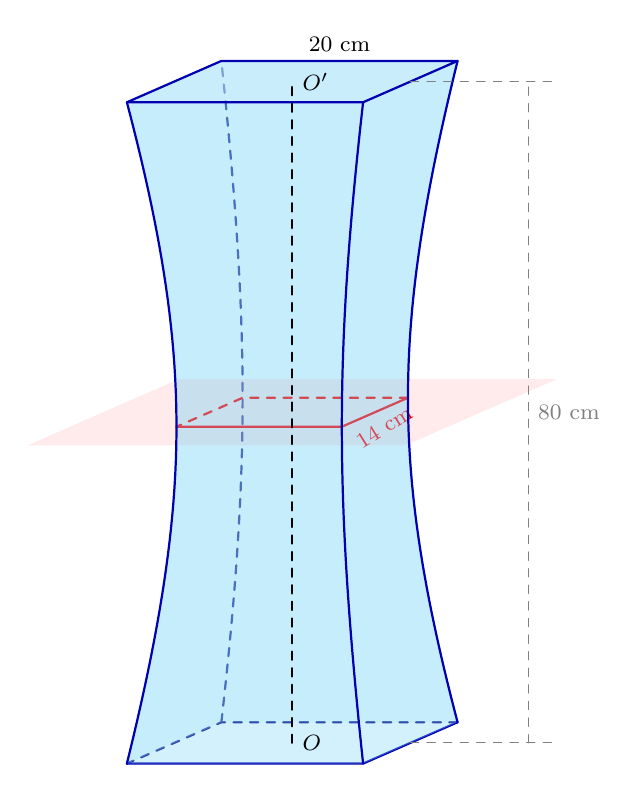
\begin{tikzpicture}[scale=0.15,yscale=.7,font=\footnotesize, line join=round, line cap=round, >=stealth,3dview/.style={x={(1cm,0cm)}, y={(0.4cm,0.25cm)}, z={(0cm,1cm)}},3dview]
			\tikzset{declare function={f(\t) = sqrt(49 + 51*(\t/40)^2);}}
			\draw[dashed, blue!50!black, thick] (10, 10, -40) -- (-10, 10, -40) -- (-10, -10, -40);
			\draw[dashed, blue!50!black, thick] plot[samples=50, domain=-40:40, variable=\t] ({-f(\t)}, {f(\t)}, \t);
			\fill[cyan!30, opacity=0.25] 
			plot[samples=50, domain=-40:40, variable=\t] ({-f(\t)}, {-f(\t)}, \t) --
			plot[samples=50, domain=40:-40, variable=\t] ({-f(\t)}, {f(\t)}, \t) -- cycle;
			\fill[cyan!30, opacity=0.25] 
			plot[samples=50, domain=-40:40, variable=\t] ({-f(\t)}, {f(\t)}, \t) --
			plot[samples=50, domain=40:-40, variable=\t] ({f(\t)}, {f(\t)}, \t) -- cycle;
			\fill[red!40, opacity=0.2] (-16, -16, 0) -- (16, -16, 0) -- (16, 16, 0) -- (-16, 16, 0) -- cycle;
			\draw[red, dashed, thick] (7, 7, 0) -- (-7, 7, 0) -- (-7, -7, 0);
			\draw[red, thick] (-7, -7, 0) -- (7, -7, 0) -- (7, 7, 0)node[below,sloped,midway]{$14$ cm};
			\draw[blue!70!black, thick] (-10, -10, -40) -- (10, -10, -40) -- (10, 10, -40);
			\fill[cyan!50, opacity=0.35] 
			plot[samples=50, domain=-40:40, variable=\t] ({-f(\t)}, {-f(\t)}, \t) --
			plot[samples=50, domain=40:-40, variable=\t] ({f(\t)}, {-f(\t)}, \t) -- cycle;
			\fill[cyan!50, opacity=0.35] 
			plot[samples=50, domain=-40:40, variable=\t] ({f(\t)}, {-f(\t)}, \t) --
			plot[samples=50, domain=40:-40, variable=\t] ({f(\t)}, {f(\t)}, \t) -- cycle;
			\draw[blue!70!black, thick] plot[samples=50, domain=-40:40, variable=\t] ({-f(\t)}, {-f(\t)}, \t);
			\draw[blue!70!black, thick] plot[samples=50, domain=-40:40, variable=\t] ({f(\t)}, {-f(\t)}, \t);
			\draw[blue!70!black, thick] plot[samples=50, domain=-40:40, variable=\t] ({f(\t)}, {f(\t)}, \t);
			\fill[cyan!30, opacity=0.6] (-10, -10, 40) -- (10, -10, 40) -- (10, 10, 40) -- (-10, 10, 40) -- cycle;
			\draw[blue!70!black, thick] (-10, -10, 40) -- (10, -10, 40) -- (10, 10, 40) -- (-10, 10, 40) -- cycle;
			\node[above] at (0, 10, 40) {$20$ cm};
			\draw[dashed, thick] (0, 0, -40)node[right]{$O$} -- (0, 0, 40)node[right]{$O'$};
			\draw[gray, dashed] (10, 0, 40) -- (22, 0, 40);
			\draw[gray, dashed] (10, 0, -40) -- (22, 0, -40);
			\draw[gray, dashed] (20, 0, -40) -- (20, 0, 40) node[midway, right] {$80$ cm};
			
		\end{tikzpicture}
	}
	\par\shortans{21{,}1}
	\loigiai{
		\immini{
			Chọn hệ trục tọa độ $Ox$ trùng với đường thẳng $OO'$, gốc tọa độ $O$ trùng với trung điểm của đoạn thẳng $OO'$.\\
			Chiều cao của chiếc đôn bằng $80$ cm nên hai mặt đáy nằm tại các mặt phẳng $x = -40$ và $x = 40$.\\
			Thiết diện cắt bởi mặt phẳng vuông góc với trục $Ox$ tại điểm có hoành độ $x$ (với $-40 \le x \le 40$) là một hình vuông.\\
			Do các cạnh bên của chiếc đôn nằm trên các đường hypebol có trục đối xứng $OO'$ nên diện tích thiết diện $S(x)$ là một hàm số bậc hai theo $x^2$ có dạng $S(x) = ax^2 + b$.\\
			Tại trung điểm của $OO'$ ($x=0$), thiết diện là hình vuông có cạnh bằng $14$ cm do đó $S(0) = 14^2 = 196 \Rightarrow b = 196$.\\
			Tại hai đáy ($x = 40$ hoặc $x = -40$), thiết diện là hình vuông có cạnh bằng $20$ cm do đó $S(40) = 20^2 = 400 \Rightarrow a \cdot 40^2 + 196 = 400 \Rightarrow 1\,600a = 204 \Rightarrow a = \dfrac{51}{400}$.}{
			\begin{tikzpicture}[
				scale=0.15, yscale=.7, font=\footnotesize, 
				line join=round, line cap=round, >=stealth,
				3dview/.style={x={(1cm,0cm)}, y={(0.4cm,0.4cm)}, z={(0cm,1cm)}},
				3dview
				]
				\tikzset{declare function={f(\t) = sqrt(49 + 51*(\t/40)^2);}}
				\draw[dashed, blue!50!black, thick] (10, 10, -40) -- (-10, 10, -40) -- (-10, -10, -40);
				\draw[dashed, blue!50!black, thick] plot[samples=50, domain=-40:40, variable=\t] ({-f(\t)}, {f(\t)}, \t);
				\fill[cyan!30, opacity=0.25] 
				plot[samples=50, domain=-40:40, variable=\t] ({-f(\t)}, {-f(\t)}, \t) --
				plot[samples=50, domain=40:-40, variable=\t] ({-f(\t)}, {f(\t)}, \t) -- cycle;
				\fill[cyan!30, opacity=0.25] 
				plot[samples=50, domain=-40:40, variable=\t] ({-f(\t)}, {f(\t)}, \t) --
				plot[samples=50, domain=40:-40, variable=\t] ({f(\t)}, {f(\t)}, \t) -- cycle;
				\fill (0,0,0) circle (10pt) node[right] {$O$};
				\fill[red!40, opacity=0.15] (-16, -16, 0) -- (16, -16, 0) -- (16, 16, 0) -- (-16, 16, 0) -- cycle;
				\draw[red, dashed, thick] (7, 7, 0) -- (-7, 7, 0) -- (-7, -7, 0);
				\draw[red, thick] (-7, -7, 0) -- (7, -7, 0) -- (7, 7, 0) node[below,sloped,midway]{$14$ cm};
				\def\x{20}
				\fill[orange!40, opacity=0.15] (-16, -16, \x) -- (16, -16, \x) -- (16, 16, \x) -- (-16, 16, \x) -- cycle;
				\fill[orange!50, opacity=0.6] ({-f(\x)}, {-f(\x)}, \x) -- ({f(\x)}, {-f(\x)}, \x) -- ({f(\x)}, {f(\x)}, \x) -- ({-f(\x)}, {f(\x)}, \x) -- cycle;
				\draw[orange!80!black, dashed, thick] ({-f(\x)}, {-f(\x)}, \x) -- ({-f(\x)}, {f(\x)}, \x) -- ({f(\x)}, {f(\x)}, \x);
				\draw[orange!80!black, thick] ({-f(\x)}, {-f(\x)}, \x) -- ({f(\x)}, {-f(\x)}, \x) -- ({f(\x)}, {f(\x)}, \x);
				\fill (0,0,\x) circle (3pt) node[below right] {$x$};
				\draw[->, orange!80!black, thick] ({f(\x)+8}, {f(\x)+2}, \x+6) node[above] {Thiết diện $S(x)$} -- ({f(\x)}, {f(\x)}, \x);
				\draw[blue!70!black, thick] (-10, -10, -40) -- (10, -10, -40) -- (10, 10, -40);
				\fill[cyan!50, opacity=0.35] 
				plot[samples=50, domain=-40:40, variable=\t] ({-f(\t)}, {-f(\t)}, \t) --
				plot[samples=50, domain=40:-40, variable=\t] ({f(\t)}, {-f(\t)}, \t) -- cycle;
				\fill[cyan!50, opacity=0.35] 
				plot[samples=50, domain=-40:40, variable=\t] ({f(\t)}, {-f(\t)}, \t) --
				plot[samples=50, domain=40:-40, variable=\t] ({f(\t)}, {f(\t)}, \t) -- cycle;
				\draw[blue!70!black, thick] plot[samples=50, domain=-40:40, variable=\t] ({-f(\t)}, {-f(\t)}, \t);
				\draw[blue!70!black, thick] plot[samples=50, domain=-40:40, variable=\t] ({f(\t)}, {-f(\t)}, \t);
				\draw[blue!70!black, thick] plot[samples=50, domain=-40:40, variable=\t] ({f(\t)}, {f(\t)}, \t);
				\draw[->, thick, black!80] (0, 0, -50) -- (0, 0, 50) node[left] {$x$};
				\fill[cyan!30, opacity=0.6] (-10, -10, 40) -- (10, -10, 40) -- (10, 10, 40) -- (-10, 10, 40) -- cycle;
				\draw[blue!70!black, thick] (-10, -10, 40) -- (10, -10, 40) -- (10, 10, 40) -- (-10, 10, 40) -- cycle;
				\node[above] at (0, 10, 40) {$20$ cm};
			\end{tikzpicture}	
		}
		\noindent Suy ra diện tích thiết diện được tính theo công thức $S(x) = \dfrac{51}{400}x^2 + 196$.\\
		Thể tích của chiếc đôn bằng
		\[V = \displaystyle\int\limits_{-40}^{40} S(x) \mathrm{\,d}x = \displaystyle\int\limits_{-40}^{40} \left(\dfrac{51}{400}x^2 + 196\right) \mathrm{\,d}x= 21\,120\,\left(\text{cm}^3\right) \approx 21{,}1\,\left(\text{dm}^3\right).\]
	}
\end{ex}


\begin{ex}%[TDMZZ17-20-TLN]%[0D0C2-3]
	Năm học 2025 – 2026 các em học sinh Tư Duy Mở đạt thành tích HSG cấp tỉnh môn Toán cực xuất sắc, với $30$ giải nhất tỉnh trong đó có $8$ thủ khoa tỉnh Toán, hơn $100$ giải nhì, hơn $180$ giải ba. Thầy Ái chọn ra $8$ học sinh giải nhất, $5$ học sinh giải nhì, $3$ học sinh giải ba để xếp ngẫu nhiên thành một hàng ngang. Gọi $p$ là xác suất để sao cho không có hai học sinh cùng giải đứng cạnh nhau. Hãy tính $10^5 p$ (\textit{không làm tròn ở các phép tính trung gian và làm tròn kết quả cuối cùng đến hàng đơn vị}).
	\par\shortans{45}
	\loigiai{
		Tổng số học sinh được chọn là $n = 8 + 5 + 3 = 16$ học sinh.\\
		Gọi $A$ là biến cố \lq\lq Xếp $16$ học sinh sao cho  không có hai học sinh cùng giải đứng cạnh nhau\rq\rq.\\
		Số cách xếp $16$ học sinh thành một hàng ngang là $n(\Omega) = 16!$.\\
		Để không có hai học sinh cùng giải đứng cạnh nhau, ta sử dụng phương pháp xếp xen kẽ.\\
		Trước hết, xếp 8 học sinh giải nhất vào 8 vị trí, có $8!$ cách.\\
		$8$ học sinh giải nhất tạo ra $9$ khoảng trống (bao gồm cả hai đầu). Gọi khoảng trống đầu hàng là khoảng trống $1$, khoảng trống cuối hàng là khoảng trống $9$, các khoảng trống giữa các học sinh giải nhất là $2$ đến $8$. Để thỏa mãn bài toán, ta xếp $5$ học sinh giải nhì, $3$ học sinh giải ba vào $9$ khoảng trống đó.\\
		Có các trường hợp $6$
		\begin{itemize}
			\item \textbf{\textbf{TH1:}} Ta xếp $5$ học sinh giải nhì, $3$ học sinh giải ba vào các khoảng trống từ $1$ đến $8$ (hoặc từ $2$ đến $9$), mỗi khoảng trống một học sinh.\\
			Ta có $2\cdot \mathrm{C}^5_8\cdot \mathrm{C}^3_3\cdot 5!\cdot 3!$ cách xếp.
			\item \textbf{\textbf{TH2:}} Ta xếp $5$ học sinh giải nhì, $3$ học sinh giải ba vào các khoảng trống từ $2$ đến $8$, khi đó có một khoảng trống có $1$ học sinh giải nhì và $1$ học sinh giải ba, các khoảng trống còn lại có một học sinh.\\
			Ta có $\mathrm{C}^1_7\cdot \mathrm{C}^4_6\cdot \mathrm{C}^2_2\cdot 2!\cdot 5!\cdot 3!$ cách xếp.
		\end{itemize}
		Ta có $n(A)=\left(2\cdot \mathrm{C}^5_8\cdot \mathrm{C}^3_3\cdot 5!\cdot 3!+\mathrm{C}^1_7\cdot \mathrm{C}^4_6\cdot \mathrm{C}^2_2\cdot 2!\cdot 5!\cdot 3!\right)\cdot 8!$.\\
		Khi đó
		$p=\cdot\mathrm{P}(A)=10^5\cdot \dfrac{n(A)}{n(\Omega)}=\dfrac{\left(2\cdot \mathrm{C}^5_8\cdot \mathrm{C}^3_3\cdot 5!\cdot 3!+\mathrm{C}^1_7\cdot \mathrm{C}^4_6\cdot \mathrm{C}^2_2\cdot 2!\cdot 5!\cdot 3!\right)\cdot 8!}{16!}=\dfrac{23}{51\,480}$.\\
		Do đó $10^5p=10^5\cdot \dfrac{23}{51\,480}\approx 45$.
	}
\end{ex}

\begin{ex}%[2H5C2-8]%[TDMZZ17]%[Trương Tường]
	Trong không gian $Oxyz$, mỗi đơn vị trên các trục tọa độ ứng với $1$ mét. Mặt phẳng $(Oxy)$ biểu diễn mặt sàn của một gara, trục $Oz$ hướng thẳng đứng lên trên. Một bức tường thẳng đứng trong gara được mô hình hóa bởi mặt phẳng $(\alpha) \colon 3x+4y-30=0$. Chiếc ô tô đang lùi chậm vào vị trí đỗ theo hướng vectơ $\vec{v}=(5;6;0)$. Ba cảm biến lùi được gắn cố định trên cản sau của ô tô. Tại thời điểm bắt đầu xét, tọa độ của ba cảm biến lần lượt là $A(1,6;1,9;0,6)$, $B(2,2;1,35;0,6)$, $C(1;2{,}25;0,6)$. Hệ thống phát tín hiệu cảnh báo \lq\lq Bíp Bíp Bíp\rq\rq~ ngay khi có ít nhất một cảm biến cách bức tường $(\alpha)$ không quá $40$ cm. Gọi $(a;b;c)$ là tọa độ của cảm biến đầu tiên đạt ngưỡng cảnh báo. Tính giá trị biểu thức $T=a+b+c$ \textit{không làm tròn ở các phép tính trung gian và làm tròn kết quả cuối cùng đến hàng phần trăm}.
	\shortans[oly]{$8{,}5$}
	\begin{center}
		\begin{tikzpicture}[scale=0.7, >=stealth, line join=round, line cap=round, font=\footnotesize]
			\def\g{-20}
			\path (0,0) coordinate (O1)
			++(\g:3) coordinate (O2)
			++({\g-90}:6) coordinate (O3)
			++($(O1)-(O2)$) coordinate (O4)		
			($(O1)!.2!(O2)$)+($.1*(O4)-.1*(O1)$) coordinate (T1)
			($(O1)!.8!(O2)$)+($.1*(O4)-.1*(O1)$) coordinate (T2)
			($(O1)!.8!(O2)$)+($.7*(O4)-.7*(O1)$) coordinate (T3)
			($(O1)!.2!(O2)$)+($.7*(O4)-.7*(O1)$) coordinate (T4)
			\foreach \l/\r/\k in {A/.25/.035, B/.5/.05, C/.75/.03}{
				($(O1)!\r!(O2)$)+($\k*(O4)-\k*(O1)$) coordinate (\l)
			}
			($(O1)!-.4!(O4)$) coordinate (L1)
			($(O2)!-.4!(O3)$) coordinate (L2)
			;
			\clip (O1)++(-3,4) rectangle ($(O3)+(4,-1)$);
			\fill [gray!20] (O1)++(-3,4) rectangle ($(O3)+(4,-1)$);
			\draw [rounded corners, fill=black!30] (O1)--(O2)--(O3)--(O4)--cycle;
			\draw [fill=black!60] (T1)--(T2)--(T3)--(T4)--cycle;
			\draw ($(O1)!.1!(T1)$)--(T1) ($(O2)!.1!(T2)$)--(T2) ($(O3)!.06!(T3)$)--(T3) ($(O4)!.06!(T4)$)--(T4);
			\foreach \x in {1,...,4}{
				\foreach \l in {A,B,C}{
					\draw [gray, rotate=\g] (\l)++(20:\x/15) arc (20:160:\x/15);
				}
			}
			\draw [fill=gray!40, very thick, draw=gray!70] ($(L1)!-1.5!(L2)+(90:1)$)--($(L2)!-1!(L1)+(90:1)$)--++(90:4)--cycle;
			\draw [line width=2mm, yellow!70!black!90] ($(L1)!-1.5!(L2)$)--($(L2)!-1!(L1)$);
			\foreach \x/\y in {A/90, B/95, C/95}{
				\draw [fill=black] (\x) circle (1pt) ++({90+\g}:.5) node {$\x$};
			}
		\end{tikzpicture}
	\end{center}
	\loigiai{
		Cảm biến thứ nhất chuyển động trên đường thẳng đi qua $A(1{,}6;1{,}9;0{,}6)$ và có vectơ chỉ phương $\vv{u}=(5;6;0)$ nên có phương trình tham số $\heva{&x=1{,}6+5t_1 \\ &y=1{,}9+6t_1 \\ &z=0{,}6}$ với $t_1$ là thời gian cảm biến chuyển động kể từ khi ở vị trí $A$ ($t_1 \ge 0$). \\
		Cảm biến thứ hai chuyển động trên đường thẳng đi qua $B(2{,}2;1{,}35,0{,}6)$ và có vectơ chỉ phương $\vv{u}=(5;6;0)$ nên có phương trình tham số $\heva{&x=2{,}2+5t_2 \\ &y=1{,}35+6t_2 \\ &z=0{,}6}$ với $t_2$ là thời gian cảm biến chuyển động kể từ khi ở vị trí $B$ ($t_2 \ge 0$). \\
		Cảm biến thứ ba chuyển động trên đường thẳng đi qua $C(1;2{,}25;0{,}6)$ và có vectơ chỉ phương $\vv{u}=(5;6;0)$ nên có phương trình tham số $\heva{&x=1+5t_3 \\ &y=2{,}25+6t_3 \\ &z=0{,}6}$ với $t_3$ là thời gian cảm biến chuyển động kể từ khi ở vị trí $C$ ($t_3 \ge 0$). \\
		Gọi $A_1$, $B_1$, $C_1$ lần lượt là vị trí của các cảm biến thứ nhất, thứ hai và thứ ba. Khi đó ta có $A_1\left(1{,}6+5t_1;1{,}9+6t_1;0{,}6\right)$, $B_1\left(2{,}2+5t_2;1{,}35+6t_2;0{,}6\right)$, $C_1\left(1+5t_3;2{,}25+6t_3;0{,}6\right)$. \\
		\textbf{Cách 1:} \\
		Khi cảm biến thứ nhất cách $(\alpha)$ một đoạn $0{,}4$ m ta có 
		\begin{eqnarray*}
			\mathrm{d}\left(A_1,(\alpha)\right)=0{,}4 &\Leftrightarrow& \dfrac{\left|3 \cdot (1{,}6+5t_1)+4 \cdot (1{,}9+6t_1)-30\right|}{\sqrt{3^2+4^2}}=0{,}4 \\
			&\Leftrightarrow& \dfrac{\left|-17{,}6+39t_1\right|}{5}=0{,}4 \\
			&\Leftrightarrow& \left|-17{,}6+39t_1\right|=2 \\
			&\Leftrightarrow& \hoac{&-17{,}6+39t_1=2 \\ &-17{,}6+39t_1=-2} \\
			&\Leftrightarrow& \hoac{&t_1=\dfrac{98}{195} \approx 0{,}5 \\ &t_1=0{,}4.}
		\end{eqnarray*}
		Do đó cảm biến thứ nhất đạt ngưỡng cảnh báo khi $t_1=0{,}4$ và tại vị trí $A_1\left(3{,}6;4{,}3;0{,}6\right)$. \\
		Khi cảm biến thứ hai cách $(\alpha)$ một đoạn $0{,}4$ m ta có 
		\begin{eqnarray*}
			\mathrm{d}\left(B_1,(\alpha)\right)=0{,}4 &\Leftrightarrow& \dfrac{\left|3 \cdot (2{,}2+5t_2)+4 \cdot (1{,}35+6t_2)-30\right|}{\sqrt{3^2+4^2}}=0{,}4 \\
			&\Leftrightarrow& \dfrac{\left|-18+39t_2\right|}{5}=0{,}4 \\
			&\Leftrightarrow& \left|-18+39t_2\right|=2 \\
			&\Leftrightarrow& \hoac{&-18+39t_2=2 \\ &-18+39t_2=-2} \\
			&\Leftrightarrow& \hoac{&t_2=\dfrac{20}{39} \\ &t_2=\dfrac{16}{39}.}
		\end{eqnarray*}
		Do đó cảm biến thứ hai đạt ngưỡng cảnh báo khi $t_2=\dfrac{16}{39}$. \\ 
		Vì $t_2>t_1$ nên cảm biến thứ hai sẽ đạt ngưỡng cảnh báo sau cảm biến thứ nhất. \\
		Khi cảm biến thứ ba cách $(\alpha)$ một đoạn $0{,}4$ m ta có 
		\begin{eqnarray*}
			\mathrm{d}\left(C_1,(\alpha)\right)=0{,}4 &\Leftrightarrow& \dfrac{\left|3 \cdot (1+5t_3)+4 \cdot (2{,}25+6t_3)-30\right|}{\sqrt{3^2+4^2}}=0{,}4 \\
			&\Leftrightarrow& \dfrac{\left|-18+39t_3\right|}{5}=0{,}4 \\
			&\Leftrightarrow& \hoac{&t_3=\dfrac{20}{39} \\ &t_3=\dfrac{16}{39}.}
		\end{eqnarray*}
		Do đó cảm biến thứ ba đạt ngưỡng cảnh báo khi $t_3=\dfrac{16}{39}$. \\ 
		Vì $t_3>t_1$ nên cảm biến thứ ba sẽ đạt ngưỡng cảnh báo sau cảm biến thứ nhất. \\
		Suy ra cảm biến thứ nhất đạt ngưỡng cảnh báo đầu tiên tại vị trí $A_1$. \\
		Ta có $a=3{,}6$; $b=4{,}3$; $c=0{,}6$. \\
		Vậy $T=a+b+c=3{,6}+4{,}3+0{,}6=8{,}5$. \\
		\textbf{Cách 2:} \\
		Thay tọa độ các điểm $A$, $B$, $C$ vào phương trình mặt phẳng $(\alpha)$ ta có 
		\begin{eqnarray*}
			&& 3 \cdot 1{,}6+4 \cdot 1{,}9-30=-17{,}6<0. \\
			&& 3 \cdot 2{,}2+4 \cdot 1{,}35-30=-18<0. \\
			&& 3 \cdot 1+4 \cdot 2{,}25-30=-18<0.
		\end{eqnarray*}
		Do đó, khi thay tọa độ các điểm $A_1$, $B_1$, $C_1$ vào phương trình mặt phẳng $(\alpha)$ ta có
		\begin{eqnarray*}
			&& 3 \cdot (1{,}6+5t_1)+4 \cdot (1{,}9+6t_1)-30=-17{,}6+39t_1 \le 0. \\
			&& 3 \cdot (1{,}6+5t_1)+4 \cdot (1{,}9+6t_1)-30=-18+39t_2 \le 0. \\
			&& 3 \cdot (1+5t_3)+4 \cdot (2{,}25+6t_3)-30=-18+39t_3 \le 0.
		\end{eqnarray*}
		Dấu \lq\lq =\rq\rq~ xảy ra khi các cảm biến chạm mặt phẳng $(\alpha)$. \\ 
		Khi các cảm biến cách mặt phẳng $(\alpha)$ một đoạn $0{,}4$ m ta có
		\begin{eqnarray*}
			&& \mathrm{d}\left(A_1,(\alpha)\right)=0{,}4 \Leftrightarrow \dfrac{\left|-17{,}6+39t_1\right|}{5}=0{,}4 \Leftrightarrow 17{,}6-39t_1=2 \Leftrightarrow t_1=0{,}4. \\
			&& \mathrm{d}\left(B_1,(\alpha)\right)=0{,}4 \Leftrightarrow \dfrac{\left|-18+39t_2\right|}{5}=0{,}4 \Leftrightarrow 18-39t_2=2 \Leftrightarrow t_2=\dfrac{16}{39} \approx 0{,}41. \\
			&& \mathrm{d}\left(C_1,(\alpha)\right)=0{,}4 \Leftrightarrow \dfrac{\left|-18+39t_3\right|}{5}=0{,}4 \Leftrightarrow 18-39t_3=2 \Leftrightarrow t_3=\dfrac{16}{39} \approx 0{,}41.
		\end{eqnarray*}
		Vì $t_1=0{,}4$ nhỏ nhất nên cảm biến thứ nhất đạt ngưỡng cảnh báo đầu tiên và tại vị trí $A_1\left(3{,}6;4{,}3;0{,}6\right)$.
	} 
\end{ex}
\begin{ex}%[0D0C2-9]%[TDMZZ17-22-TLN]%[Nguyễn Văn Sang]
	Một bạn học sinh tên Hùng dùng $5$ màu khác nhau (trong đó có màu đỏ) để tô cho $7$ hình tròn $A, B, C, D, E, F, G$ như hình vẽ bên dưới, sao cho mỗi hình tròn tô một màu. Hai cách tô màu được gọi là khác nhau nếu xét theo thứ tự $A, B, C, D, E, F, G$ có ít nhất một vị trí cho màu khác nhau.
	%--- Bắt đầu vẽ hình minh hoạ đề bài ---%
	\begin{center}
		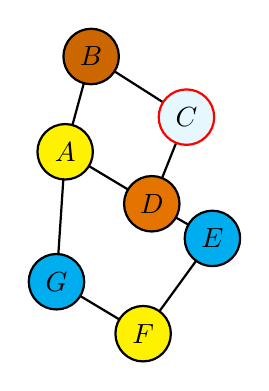
\begin{tikzpicture}[scale=1.1, font=\sffamily, line join=round, line cap=round, >=stealth]
			% Định nghĩa tọa độ các đỉnh
			\coordinate (B) at (0, 2);
			\coordinate (A) at (-0.3, 0.9);
			\coordinate (C) at (1.1, 1.3);
			\coordinate (D) at (0.7, 0.3);
			\coordinate (G) at (-0.4, -0.6);
			\coordinate (E) at (1.4, -0.1);
			\coordinate (F) at (0.6, -1.2);
			
			% Vẽ các cạnh nối
			\draw[thick] (B) -- (A);
			\draw[thick] (B) -- (C);
			\draw[thick] (C) -- (D);
			\draw[thick] (A) -- (D);
			\draw[thick] (A) -- (G);
			\draw[thick] (D) -- (E);
			\draw[thick] (G) -- (F);
			\draw[thick] (E) -- (F);
			
			% Vẽ các hình tròn
			\draw[fill=orange!80!black, draw=black, thick] (B) circle (0.32) node {\color{black} $B$};
			\draw[fill=yellow, draw=black, thick] (A) circle (0.32) node {\color{black} $A$};
			\draw[fill=cyan!10, draw=red, thick] (C) circle (0.32) node {\color{black} $C$};
			\draw[fill=orange!90!black, draw=black, thick] (D) circle (0.32) node {\color{black} $D$};
			\draw[fill=cyan, draw=black, thick] (E) circle (0.32) node {\color{black} $E$};
			\draw[fill=cyan, draw=black, thick] (G) circle (0.32) node {\color{black} $G$};
			\draw[fill=yellow, draw=black, thick] (F) circle (0.32) node {\color{black} $F$};
		\end{tikzpicture}
	\end{center}
	%--- Kết thúc vẽ hình minh hoạ ---%
	Gọi $T$ là số cách tô màu thoả mãn đồng thời các điều kiện sau:
	\begin{itemize}
		\item Có đúng $1$ ô được tô màu đỏ.
		\item Hai ô được nối với nhau bởi đoạn thẳng được tô màu khác nhau.
	\end{itemize}
	Hãy tính $T$?
	\shortans[oly]{$ 5652 $}
	\loigiai{
		
		\textbf{PHƯƠNG PHÁP XÓA ĐỈNH VÀ 3 MÔ HÌNH TÔ MÀU CƠ BẢN ($4$ MÀU)}
		\begin{itemize}
			\item \textbf{Tư duy cốt lõi:} Đề bài yêu cầu \textbf{có đúng $1$ ô màu đỏ}. Nếu ta chọn cố định ô đó và tô màu đỏ, thì $6$ ô còn lại bắt buộc phải tô bằng $4$ màu còn lại (tuyệt đối không được dùng lại màu đỏ).
			\item Khi đó, ô màu đỏ sẽ chắc chắn khác màu với các ô xung quanh. Ta có thể "gạch bỏ" (xóa) ô màu đỏ và các đoạn thẳng dính với nó đi.
			\item Đồ thị vỡ ra thành các mảng đơn giản. Ta đi đếm số cách tô các mảng này bằng $4$ màu thông qua $3$ Bổ đề sau:
			\item \textbf{Bổ đề 1 - Mô hình Đường thẳng ($n$ đỉnh):}
			\begin{itemize}
				\item Đỉnh số 1 có $4$ cách chọn màu.
				\item Các đỉnh nối tiếp theo mỗi đỉnh chỉ cần né màu của đỉnh liền trước, nên có $3$ cách.
				\item Số cách tô một đường thẳng $n$ đỉnh là: $\displaystyle 4 \times 3^{n-1}$.
			\end{itemize}
			\item \textbf{Bổ đề 2 - Mô hình Vòng $4$ đỉnh khép kín ($C_4$): Gọi là $1-2-3-4-1$}
			\begin{itemize}
				\item Đỉnh 1 có $4$ cách; Đỉnh 2 có $3$ cách. Xét Đỉnh 3 (đối diện Đỉnh 1):
				\item \textit{Nếu Đỉnh 3 cùng màu Đỉnh 1 (1 cách):} Khi đó Đỉnh 4 chỉ cần khác 1 màu chung này $\Rightarrow$ có $3$ cách. (Gồm $4 \times 3 \times 1 \times 3 = 36$ cách).
				\item \textit{Nếu Đỉnh 3 khác màu Đỉnh 1 (2 cách):} Khi đó Đỉnh 4 phải né 2 màu khác nhau $\Rightarrow$ có $2$ cách. (Gồm $4 \times 3 \times 2 \times 2 = 48$ cách).
				\item Tổng số cách tô vòng 4 đỉnh: $\displaystyle 36 + 48 = 84$ cách.
			\end{itemize}
			\item \textbf{Bổ đề 3 - Mô hình Vòng $5$ đỉnh khép kín ($C_5$): Gọi là $1-2-3-4-5-1$}
			\begin{itemize}
				\item Đỉnh 1 (4 cách), Đỉnh 2 (3 cách). Xét Đỉnh 3:
				\item \textit{TH 3a: Đỉnh 3 cùng màu Đỉnh 1 (1 cách):} Khi đó Đỉnh 4 (3 cách) $\Rightarrow$ Đỉnh 5 kề Đỉnh 4 và Đỉnh 1 (hai màu này đã khác nhau) $\Rightarrow$ Đỉnh 5 có $2$ cách. (Nhóm này có $4 \times 3 \times 1 \times 3 \times 2 = 72$ cách).
				\item \textit{TH 3b: Đỉnh 3 khác màu Đỉnh 1 (2 cách):} Ta xét tiếp Đỉnh 4:
				\begin{itemize}
					\item Đỉnh 4 cùng màu Đỉnh 1 (1 cách) $\Rightarrow$ Đỉnh 5 kề hai đỉnh cùng màu nên có $3$ cách. $\Rightarrow (1 \times 3 = 3$ cách$)$.
					\item Đỉnh 4 khác màu Đỉnh 1 (2 cách) $\Rightarrow$ Đỉnh 5 kề hai đỉnh khác màu nên có $2$ cách. $\Rightarrow (2 \times 2 = 4$ cách$)$.
				\end{itemize}
				\item Nhóm 3b có: $4 \times 3 \times 2 \times (3 + 4) = 168$ cách.
				\item Tổng số cách tô vòng 5 đỉnh: $\displaystyle 72 + 168 = 240$ cách.
			\end{itemize}
		\end{itemize}
		Dựa vào tính đối xứng của hình vẽ qua trục dọc, các đỉnh đối xứng nhau có vai trò giống hệt nhau. Ta chia làm 4 trường hợp đặt ô màu đỏ.
		\begin{itemize}
			\item \textbf{Trường hợp 1: Ô đỏ nằm tại $B$ hoặc $C$ (Có $2$ khả năng)}
			\immini
			{\begin{itemize}
					\item Giả sử chọn đỉnh $B$ tô màu đỏ. Xóa đỉnh $B$ đi.
					\item Nhìn vào hình vẽ (đã làm mờ B), ta thấy $6$ đỉnh còn lại dính nhau tạo thành một \textbf{vòng 5 đỉnh} ($A-G-F-E-D-A$) và một "cái râu" $C$ bám vào $D$.
					\item Tô màu vòng $5$ đỉnh ($C_5$) bằng $4$ màu: Áp dụng Bổ đề 3, ta có $\displaystyle 240$ cách.
					\item Đỉnh râu $C$ chỉ bám duy nhất vào $D$, nên $C$ có $3$ cách (né màu của $D$).
					\item Số cách tô khi $B$ đỏ là: $\displaystyle 240 \times 3 = 720$ cách.
					\item Nhân đôi lên cho cả trường hợp $C$ đỏ, ta có: $\displaystyle 2 \times 720 = 1440$ cách.
			\end{itemize}}
			{ 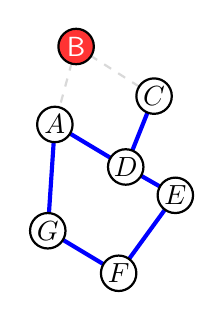
\begin{tikzpicture}[scale=0.9, font=\sffamily, thick]
					\coordinate (B) at (0, 2); \coordinate (A) at (-0.3, 0.9);
					\coordinate (C) at (1.1, 1.3); \coordinate (D) at (0.7, 0.3);
					\coordinate (G) at (-0.4, -0.6); \coordinate (E) at (1.4, -0.1);
					\coordinate (F) at (0.6, -1.2);
					\draw[gray!30, dashed] (B)--(A) (B)--(C);
					\draw[blue, line width=1.5pt] (C)--(D) (A)--(D) (A)--(G) (D)--(E) (G)--(F) (E)--(F);
					\draw[fill=red!80, draw=black] (B) circle (0.25) node[text=white] {B};
					\foreach \p in {A,C,D,E,G,F} \draw[fill=white, draw=black] (\p) circle (0.25) node {$\p$};
			\end{tikzpicture}}
			\item \textbf{Trường hợp 2: Ô đỏ nằm tại $A$ hoặc $D$ (Có $2$ khả năng)}
			\immini
			{ \begin{itemize}
					\item Giả sử chọn $A$ màu đỏ. Xóa đỉnh $A$ đi.
					\item Quan sát hình, việc xóa $A$ làm đứt hẳn liên kết vòng, đồ thị duỗi thẳng ra thành \textbf{đúng một đường thẳng} gồm $6$ đỉnh: $B - C - D - E - F - G$.
					\item Tô màu đường thẳng $6$ đỉnh bằng $4$ màu: Áp dụng Bổ đề 1, ta có $\displaystyle 4 \times 3^5 = 972$ cách.
					\item Nhân đôi lên cho cả trường hợp $D$ đỏ, ta có: $\displaystyle 2 \times 972 = 1944$ cách.
			\end{itemize}}
			{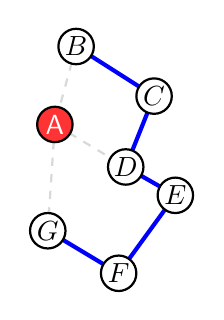
\begin{tikzpicture}[scale=0.9, font=\sffamily, thick]
					\coordinate (B) at (0, 2); \coordinate (A) at (-0.3, 0.9);
					\coordinate (C) at (1.1, 1.3); \coordinate (D) at (0.7, 0.3);
					\coordinate (G) at (-0.4, -0.6); \coordinate (E) at (1.4, -0.1);
					\coordinate (F) at (0.6, -1.2);
					\draw[gray!30, dashed] (B)--(A) (A)--(D) (A)--(G);
					\draw[blue, line width=1.5pt] (B)--(C) (C)--(D) (D)--(E) (E)--(F) (F)--(G);
					\draw[fill=red!80, draw=black] (A) circle (0.25) node[text=white] {A};
					\foreach \p in {B,C,D,E,G,F} \draw[fill=white, draw=black] (\p) circle (0.25) node {$\p$};
			\end{tikzpicture}}
			\item \textbf{Trường hợp 3: Ô đỏ nằm tại $F$ (Có duy nhất $1$ khả năng)}
			\immini{ \begin{itemize}
					\item Giả sử tô $F$ màu đỏ và xóa nó.
					\item Đồ thị phía trên còn lại một \textbf{vòng 4 đỉnh} ($A-B-C-D-A$) và hai "cái râu" $G$ (bám vào $A$) và $E$ (bám vào $D$).
					\item Tô màu vòng $4$ đỉnh ($C_4$) bằng $4$ màu: Áp dụng Bổ đề 2, ta có $\displaystyle 84$ cách.
					\item Hai cái râu $G, E$ mọc ra từ $A, D$ đã tô màu, nên mỗi râu tự do chọn $3$ cách.
					\item Tổng số cách tô khi $F$ đỏ là: $\displaystyle 1 \times 84 \times 3 \times 3 = 756$ cách.
			\end{itemize}}
			{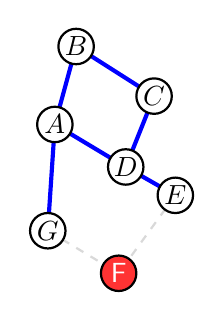
\begin{tikzpicture}[scale=0.9, font=\sffamily, thick]
					\coordinate (B) at (0, 2); \coordinate (A) at (-0.3, 0.9);
					\coordinate (C) at (1.1, 1.3); \coordinate (D) at (0.7, 0.3);
					\coordinate (G) at (-0.4, -0.6); \coordinate (E) at (1.4, -0.1);
					\coordinate (F) at (0.6, -1.2);
					\draw[gray!30, dashed] (G)--(F) (E)--(F);
					\draw[blue, line width=1.5pt] (B)--(A) (B)--(C) (C)--(D) (A)--(D) (A)--(G) (D)--(E);
					\draw[fill=red!80, draw=black] (F) circle (0.25) node[text=white] {F};
					\foreach \p in {B,A,C,D,E,G} \draw[fill=white, draw=black] (\p) circle (0.25) node {$\p$};
			\end{tikzpicture}}
			\item \textbf{Trường hợp 4: Ô đỏ nằm tại $G$ hoặc $E$ (Có $2$ khả năng)}
			\immini
			{\begin{itemize}
					\item Giả sử chọn $G$ màu đỏ và xóa đi.
					\item Đồ thị còn lại gồm một \textbf{vòng 4 đỉnh} ($A-B-C-D-A$) và một đoạn thẳng nối đuôi chạy ra ngoài $D-E-F$ (Đỉnh $E$ bám vào $D$, đỉnh $F$ bám vào $E$).
					\item Tô vòng khép kín $C_4$: Có $\displaystyle 84$ cách (Bổ đề 2).
					\item Tô dọc theo đường thẳng $D-E-F$: Đỉnh $E$ né $D$ ($3$ cách), đỉnh $F$ né $E$ ($3$ cách).
					\item Số cách tô khi $G$ đỏ là: $\displaystyle 84 \times 3 \times 3 = 756$ cách.
					\item Nhân đôi lên cho cả trường hợp $E$ đỏ, ta có: $\displaystyle 2 \times 756 = 1512$ cách.
			\end{itemize}}
			{ 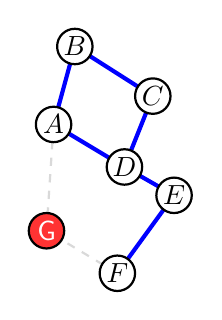
\begin{tikzpicture}[scale=0.9, font=\sffamily, thick]
					\coordinate (B) at (0, 2); \coordinate (A) at (-0.3, 0.9);
					\coordinate (C) at (1.1, 1.3); \coordinate (D) at (0.7, 0.3);
					\coordinate (G) at (-0.4, -0.6); \coordinate (E) at (1.4, -0.1);
					\coordinate (F) at (0.6, -1.2);
					\draw[gray!30, dashed] (A)--(G) (F)--(G);
					\draw[blue, line width=1.5pt] (B)--(A) (B)--(C) (C)--(D) (A)--(D) (D)--(E) (E)--(F);
					\draw[fill=red!80, draw=black] (G) circle (0.25) node[text=white] {G};
					\foreach \p in {B,A,C,D,E,F} \draw[fill=white, draw=black] (\p) circle (0.25) node {$\p$};
			\end{tikzpicture}}
			\item \textbf{Tổng kết bài toán}\\
			Vì $4$ trường hợp trên là độc lập và bao quát toàn bộ các khả năng chọn vị trí ô màu đỏ. Áp dụng quy tắc cộng, tổng số cách tô màu thỏa mãn yêu cầu bài toán là:
			\[ \displaystyle T = 1440 + 1944 + 756 + 1512 = 5652 \text{ cách.} \]
		\end{itemize}
	}
\end{ex}